\section{Техническое задание}
\subsection{Основание для разработки}

Основанием для разработки является задание на выпускную квалификационную работу бакалавра "<Программный продукт для администрирования и разработки баз данных">.

\subsection{Цель и назначение разработки}

Разрабатываемая программно-информационная система предназначена для локального хранения, редактирования, поиска и визуализации табличных данных с использованием команд SQL-подобного формата.

Программа реализует функции создания базы данных и таблиц с указанными типами данных, а также предоставляет операции вставки, удаления, выборки и обновления данных на основе пользовательских условий. Встроенный графический интерфейс позволяет отображать содержимое таблиц в удобной форме.

Программа ориентирована на студентов, преподавателей и разработчиков, нуждающихся в простом и наглядном инструменте работы с небольшими объемами структурированных данных без необходимости установки полноценных СУБД.

Задачами данной разработки являются:
\begin{enumerate}
\item Разработка реляционной модели хранения данных с использованием таблиц.
\item Реализация операций CREATE, INSERT, SELECT, UPDATE, DELETE.
\item Создание пользовательского интерфейса для взаимодействия с базой данных и ввода команд.
\item Обеспечение сохранения баз данных на диск и их последующей загрузки.
\item Обработка пользовательских ошибок с предоставлением понятных уведомлений и сообщений.
\end{enumerate}

\subsection{Требования пользователя к программной системе}

\subsubsection{Требования к данным программной системы}

Программная система должна обеспечивать хранение табличных структур с поддержкой различных типов данных. Внутреннее представление таблиц и баз данных реализуется в оперативной памяти с возможностью сохранения на диск.

Основные требования:
\begin{enumerate}
	\item Данные хранятся в виде таблиц, каждая из которых имеет уникальное имя, перечень столбцов и определённые типы данных для каждого столбца.
	\item Поддерживаются следующие типы данных:
	\begin{itemize}
		\item integer -- целочисленные значения;
		\item float -- вещественные числа с плавающей точкой; 
		\item string -- строковые значения.
	\end{itemize}
	\item Все таблицы сгруппированы по базам данных. Каждая база данных представлена в виде отдельного файла с расширением .db, хранящегося на диске.
	\item Таблицы допускают следующие действия над данными: вставка новых строк, выборка с условиями, обновление и удаление строк.
\end{enumerate}

\subsubsection{Требования к интерфейсу}

Графический интерфейс предоставляет пользователю простые и интуитивные средства для взаимодействия с системой.

Обязательные элементы интерфейса:
\begin{enumerate}
	\item Текстовое поле для ввода SQL-подобных команд.		
	\item Таблица для визуализации результатов выборки данных.	
	\item Меню для выполнения операций загрузки и сохранения базы данных.	
	\item Система уведомлений для отображения ошибок или успешных действий.
\end{enumerate}

\subsubsection{Функциональные требования к программной системе}

Программа должна реализовать следующие функциональные возможности:
\begin{enumerate}
	\item Создание базы данных: команда create database <имя> создаёт новую базу данных и делает её активной; при создании новой базы автоматически сохраняется предыдущая, если таковая была выбрана.
	\item Создание таблиц: команда create table <имя> <столбец1> <тип1> <столбец2> <тип2>... создаёт таблицу в текущей базе данных; структура таблицы включает в себя названия столбцов и типы хранящихся в них данных.
	\item Вставка данных: команда insert into <таблица> values <значение1> <значение2>... добавляет новую строку в указанную таблицу.
	\item Выборка данных: команда select <столбцы|*> from <таблица> [where <условие>] выводит строки, удовлетворяющие условию, в таблицу интерфейса.
	\item Удаление данных: команда delete from <таблица> [where <условие>] удаляет строки, соответствующие условию.
	\item Обновление данных: команда update <таблица> set <столбец1> <значение1> ... [where <условие>] изменяет значения в указанных столбцах.
	\item Сохранение/загрузка базы данных: меню File -> Save сохраняет текущую базу в файл; меню File -> Open загружает ранее сохранённую базу.
	\item Обработка пользовательских ошибок: система должна проверять корректность команд и типов данных, выводя информативные сообщения об ошибках.
\end{enumerate}

\subsection{Моделирование вариантов использования}

Для разрабатываемой СУБД была реализована модель, которая обеспечивает наглядное представление вариантов использования программы.

Диаграмма прецедентов описывает функциональное назначение разрабатываемой программы. Проектируемая система представляется в виде ряда прецедентов, предоставляемых системой актерам или сущностям, которые взаимодействуют с системой. Актером или действующим лицом является сущность, взаимодействующая с системой извне. Прецедент служит для описания набора действий, которые система предоставляет актеру.

На основании анализа предметной области в программе должны быть реализованы следующие прецеденты:
\begin{enumerate}
	\item Создание базы данных.
	\item Создание таблицы.
	\item Вставка записи в таблицу.
	\item Выборка данных из таблицы.
	\item Удаление данных из таблицы.
	\item Обновление записей в таблице.
	\item Сохранение базы данных.
	\item Загрузка базы данных.
\end{enumerate}

На рисунке ~\ref{fig:prec} представлена диаграмма прецедентов для разрабатываемой программы.

\begin{figure}[H]
	\centering
	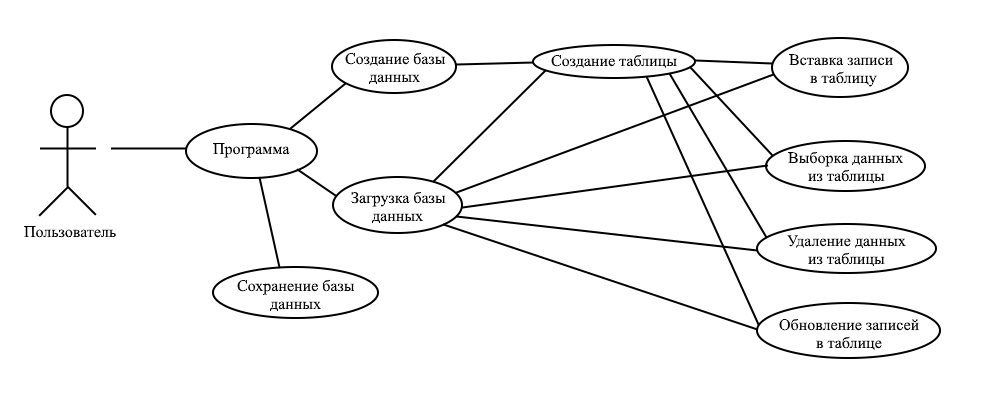
\includegraphics[width=1\linewidth]{images/prec}
	\caption{Диаграмма прецедентов}
	\label{fig:prec}
\end{figure}

\subsubsection{Сценарии прецедентов программы}

\paragraph{Создание базы данных}

Заинтересованные лица и их требования: пользователь желает создать новую базу данных для хранения информации о таблицах, с возможностью дальнейшего сохранения, загрузки и редактирования.

Предусловие: программа запущена, текущая база данных не выбрана или пользователь хочет создать новую.

Постусловие: создана база данных; пользователь может создавать в ней таблицы и добавлять данные.

Основной успешный сценарий:
\begin{enumerate}
	\item Пользователь вводит в поле ввода команду в формате create database <имя базы>.	
	\item Пользователь нажимает на кнопку Run.	
	\item Программа проверяет наличие базы с таким именем в текущем сеансе и на диске:
	\begin{itemize}
		\item если база уже существует и не открыта, выводится предупреждение;	
		\item если открыта другая база данных — запрашивается подтверждение на создание новой.
	\end{itemize}
	\item Если ранее была открыта другая база, она сериализуется и сохраняется, если пользователь подтвердил сохранение.	
	\item Создаётся новая база данных, в которой инициализируются пустой список таблиц и идентификатор имени.	
	\item Созданная база данных устанавливается как текущий рабочий объект.
	\item Выводится сообщение об успешном создании базы данных.	
\end{enumerate}

\paragraph{Создание таблицы}

Заинтересованные лица и их требования: пользователь хочет определить структуру новой таблицы, включающей названия и типы столбцов, в рамках активной базы данных.

Предусловие: открыта и активна база данных, в которой ещё не существует таблицы с заданным именем.

Постусловие: создана таблица с заданными колонками и типами данных и добавлена в базу данных.

Основной успешный сценарий:
\begin{enumerate}
	\item Пользователь вводит в поле ввода команду create table <имя таблицы> <название столбца1> <тип1> <название столбца2> <тип2>... .
	\item Пользователь нажимает на кнопку Run.	
	\item Программа выполняет предварительный разбор команды, разделяя имя таблицы и пары название + тип.	
	\item Программа проверяет:
	\begin{itemize}
		\item корректность имени таблицы;	
		\item уникальность имён столбцов;	
		\item допустимость типов (integer, float, string).
	\end{itemize}
	\item При наличии ошибок система выводит понятное сообщение с подсказкой и отменяет создание.	
	\item При успешной валидации создаётся таблица, в которую записываются:
	\begin{itemize}
		\item список имён столбцов;	
		\item соответствующие типы данных;	
		\item пустой список строк.
	\end{itemize}	
	\item Таблица добавляется в базу данных.	
	\item Выводится сообщение об успешном создании таблицы.
\end{enumerate}

\paragraph{Вставка записи в таблицу}

Заинтересованные лица и их требования: пользователь хочет добавить новую строку данных в выбранную таблицу, соблюдая типы данных, заданные при создании таблицы.

Предусловие: в базе данных должна существовать хотя бы одна таблица. Пользователь знает структуру таблицы и допустимые типы данных.

Постусловие: новая запись добавлена в таблицу, данные сериализуются в оперативной памяти. В случае ошибки типизации — запись не производится.

Основной успешный сценарий:
\begin{enumerate}
	\item Пользователь вводит в поле ввода команду insert into <имя таблицы> values <значение1> <значение2>... .	
	\item Пользователь нажимает на кнопку Run.	
	\item Программа определяет таблицу по имени и извлекает информацию о столбцах и их типах.	
	\item Каждое значение из команды обрабатывается через синтаксический разбор и приводится к нужному типу.	
	\item Программа проверяет:
	\begin{itemize}
		\item соответствие количества значений числу столбцов;	
		\item соответствие типов.
	\end{itemize}
	\item Если проверка не пройдена, отображается окно с ошибкой и описанием проблемы.	
	\item При успешной валидации в таблицу добавляется новая строка с указанными значениями.	
	\item Таблица обновляется в графическом интерфейсе.
\end{enumerate}

\paragraph{Выборка данных из таблицы}

Заинтересованные лица и их требования: пользователь хочет получить данные из таблицы, отфильтрованные по определённым условиям, с выбором конкретных столбцов.

Предусловие: существует хотя бы одна таблица с данными. Пользователь знает названия столбцов и возможные условия фильтрации.

Постусловие: на экране появляется таблица с данными, удовлетворяющими условию и содержащая выбранные столбцы.

Основной успешный сценарий:
\begin{enumerate}
	\item Пользователь вводит в поле ввода команду select <столбец1> <столбец2> ... from <имя таблицы> [where <условие>].
	\item Пользователь нажимает на кнопку Run.	
	\item Программа разбирает команду:
	\begin{itemize}
		\item выделяет список столбцов;		
		\item определяет имя таблицы;		
		\item извлекает и парсит условие (если есть).
	\end{itemize}
	\item Программа извлекает из таблицы данные, удовлетворяющие фильтру.	
	\item Выбираются значения только указанных пользователем столбцов.	
	\item Таблица обновляется в графическом интерфейсе: устанавливаются выбранные заголовки, выводятся строки.	
	\item Если запрос некорректен (неверный синтаксис или ошибка в условии), выводится понятное сообщение об ошибке.
\end{enumerate}

\paragraph{Удаление данных из таблицы}

Заинтересованные лица и их требования: пользователь желает удалить одну или несколько строк таблицы, удовлетворяющих заданному условию.

Предусловие: существует таблица с данными. Пользователь знает структуру данных и условия фильтрации.

Постусловие: из таблицы удалены строки, для которых выполняется условие. Оставшиеся строки остаются без изменений.

Основной успешный сценарий:
\begin{enumerate}
	\item Пользователь вводит в поле ввода команду delete from <имя таблицы> [where <условие>].
	\item Пользователь нажимает на кнопку Run.		
	\item Программа разбирает команду, извлекает имя таблицы и условие (если указано).	
	\item Условие обрабатывается через ast, компилируется в функцию фильтрации.	
	\item Программа проходит по каждой строке таблицы: если условие верно, то строка исключается.	
	\item По завершении удаления данные в таблице обновляются.	
	\item Таблица обновляется в графическом интерфейсе.
\end{enumerate}

\paragraph{Обновление записей в таблице}

Заинтересованные лица и их требования: пользователь желает изменить значения одного или нескольких столбцов для всех строк, удовлетворяющих заданному условию.

Предусловие: существует таблица с данными. Указанные столбцы существуют, новые значения допустимы по типу.

Постусловие: в таблице изменены данные в указанных столбцах для строк, удовлетворяющих условию.

Основной успешный сценарий:
\begin{enumerate}
	\item Пользователь вводит в поле ввода команду update <имя таблицы> set <столбец1> <значение1> ... [where <условие>].
	\item Пользователь нажимает на кнопку Run.		
	\item Программа извлекает имя таблицы, пары столбец + значение и условие (если указано).	
	\item Каждое новое значение разбирается и приводится к типу, заданному для соответствующего столбца.	
	\item Программа применяет условие ко всем строкам: если условие выполняется, то обновляются нужные поля.	
	\item Если хотя бы одно значение имеет несовместимый тип, операция прерывается.	
	\item Данные в таблице обновляются.
	\item Таблица обновляется в графическом интерфейсе.
\end{enumerate}

\paragraph{Сохранение базы данных}

Заинтересованные лица и их требования: пользователь хочет сохранить текущую базу данных с таблицами и данными на диск, чтобы в будущем загрузить её.

Предусловие: выбрана и активна база данных.

Постусловие: файл .db с сериализованным объектом базы сохранён на диск в папке databases/.

Основной успешный сценарий:
\begin{enumerate}
	\item Пользователь выбирает File -> Save из меню.	
	\item Программа проверяет, выбрана ли активная база. Если нет — выводит сообщение об ошибке.	
	\item Используется pickle для сериализации объекта базы в байтовый поток.	
	\item Байты сохраняются в файл databases/<имя базы>.db.	
	\item Программа подтверждает успешное сохранение.
\end{enumerate}

\paragraph{Загрузка базы данных}

Заинтересованные лица и их требования: пользователь хочет загрузить ранее сохранённую базу, чтобы продолжить работу с таблицами.

Предусловие: файл базы данных ранее был сохранён и доступен на диске.

Постусловие: объект базы данных загружен в память, пользователь может выполнять над ним операции.

Основной успешный сценарий:
\begin{enumerate}
	\item Пользователь выбирает File -> Open из меню.	
	\item Открывается диалог выбора файла. Пользователь выбирает .db файл.	
	\item Текущая активная база данных сохраняется в свой файл.
	\item Программа десериализует объект с помощью pickle.	
	\item Загруженный объект становится текущей активной базой.	
\end{enumerate}

\subsection{Требования к оформлению документации}

Разработка программной документации и программного изделия должна производиться согласно ГОСТ 19.102-77 и ГОСТ 34.601-90. Единая система программной документации.
